\usepackage{etex} %эта магическая херь избавляет от переполнения регистров TeX а!!!

\mode<article>{\usepackage{fullpage}}
\mode<presentation>{
    \usetheme{Madrid}
    \useoutertheme{shadow}
} 

\usepackage[utf8]{inputenc}
\usepackage[russian]{babel}
\usepackage{indentfirst}
\usepackage{graphicx}

\usepackage{amsmath}
\usepackage{amsfonts}
\usepackage{amsthm}
%\usepackage{algorithm}
%\usepackage{algorithmic}

%\usepackage[all]{xy}

\date{Лекция по дисциплине <<методы и средства защиты компьютерной информации>> (\today)}
\author[М.~М.~Шихов]{Михаил Шихов \\ \texttt{\underline{m.m.shihov@gmail.com}}}

%%для рисования графов пакетом xy-pic
%\entrymodifiers={++[o][F-]}

%%для псевдокода алгоритмов (algorithm,algorithmic)
%\renewcommand{\algorithmicrequire}{\textbf{Вход:}}
%\renewcommand{\algorithmicensure}{\textbf{Выход:}}
%\renewcommand{\algorithmiccomment}[1]{// #1}
%\floatname{algorithm}{Псевдокод}

%\setbeamercolor{alerted text}{fg=-green} %gyan, blue, green, -green



\title[Внедрение кода]{Внедрение вредоносного программного кода}


\begin{document}

\mode<article>{\maketitle\tableofcontents}
\frame<presentation>{\titlepage}
\begin{frame}<presentation>[allowframebreaks]
    \frametitle{Содержание}
    \tableofcontents
\end{frame}


\section{Угрозы}


\subsection{Перехват потока выполнения} 

\begin{frame}[fragile]
    \frametitle{Переполнение буфера}
    \framesubtitle{Срыв стека}
    
\shorthandoff{"}
\begin{semiverbatim}
#include <stdio.h>
#include <string.h>

void badStrcpy(char *input) \{
    char buf[16];
    strcpy(buf, input);
    printf(buf);
\}

int main(int argc, char *argv[]) \{
    badStrcpy(argv[1]);
\}
\end{semiverbatim}
\shorthandon{"}
\end{frame}


\begin{frame}[fragile]
    \frametitle{Переполнение буфера}
    \framesubtitle{Детали: \verb"int main(int argc, char *argv[])"}
    
\shorthandoff{"}
\begin{columns}
    \column{0.45\textwidth}
\begin{semiverbatim}
//int main(argc, argv) \{
004012fe:\alert<2->{push ebp
        mov ebp,esp //...
}//  badStrcpy(argv[1]);
        \alert<3->{mov eax, [ebp+0xC]
        add eax, 0x4
        mov eax, [eax]
        push eax
}        call 0x4012d0
//\}
00401338:mov eax, 0
        mov esp, ebp
        pop ebp
        ret
\end{semiverbatim}
    \column{0.54\textwidth}
        \begin{block}{}
            \begin{tabular}[c]{lll}
                22FF04  &          &\\
                22FF08  &          &\\
                22FF0C  &          &\\
                22FF10  &          &\\
                22FF14  &          &\\
                22FF18  &          &\\
                22FF1C  &          &\\
                22FF20  &          &\\
                22FF24  &\only<3->{004A25E1}  
                                   &\only<3->{\&argv[1],input}\\
                22FF28  &\only<2->{0022FF68}  
                                   &\only<2->{[ebp]}\\
                22FF2C  &004010B6  &\&cp(main)\\
                22FF30  &00000004  &argc\\
                22FF34  &003F17D8  &\&argv
            \end{tabular}
    \end{block}
\end{columns}
\shorthandon{"}
\end{frame}

\begin{frame}[fragile]
    \frametitle{Переполнение буфера}
    \framesubtitle{Детали: \verb"void badStrcpy(char *input)"}
    
\shorthandoff{"}
\begin{columns}
    \column{0.40\textwidth}
\begin{semiverbatim}
004012d0:
\alert<2->{    push ebp
    mov ebp,esp
    sub esp,0x18
}\alert<3->{    mov eax,[ebp+0x8]
    mov [esp+0x4],eax
    lea eax,[ebp-0x10]
    mov [esp],eax
}\alert<4->{    call 0x401b48<strcpy>
}\alert<5->{    lea eax,[ebp-0x10]
    mov [esp],eax
}\alert<6->{    call 0x401b40<printf>
}\alert<7->{    leave 
}    ret 
\end{semiverbatim}
    \column{0.6\textwidth}
    \begin{block}{}
        \begin{tabular}[c]{lll}
            22FF04  &\only<2>{xxxxxxxx}\only<3-6>{0022FF0C}
                                &\only<2-6>{[esp]}\only<3,5>{,\&buf[0]}\\
            22FF08  &\only<2>{xxxxxxxx}\only<3-6>{004A25E1}
                                &\only<3>{input}\\
            22FF0C  &\only<2-3>{xxxxxxxx}\only<4-6>{h e l l}
                                &\only<2-6>{buf[0]..buf[3]}\\
            22FF10  &\only<2-3>{xxxxxxxx}\only<4-6>{o , \_ W}
                                &\only<2-6>{buf[4]..buf[7]}\\
            22FF14  &\only<2-3>{xxxxxxxx}\only<4-6>{o r l d}
                                &\only<2-6>{buf[8]..buf[B]}\\
            22FF18  &\only<2-3>{xxxxxxxx}\only<4-6>{! ! ! 00}
                                &\only<2-6>{buf[C]..buf[F]}\\
            22FF1C  &\only<2-6>{0022FF28}
                                &\only<2-6>{[ebp]}\\
            
            22FF20  &00401338  &\only<7>{[esp],}\&cp(badStrcpy)\\
            22FF24  &004A25E1  &\&argv[1],input\\
            22FF28  &0022FF68  &\only<7>{[ebp]}\only<1-6>{$\text{ebp}_\text{main}$}\\
            22FF2C  &004010B6  &\&cp(main)\\
            22FF30  &00000004  &argc\\
            22FF34  &003F17D8  &\&argv
        \end{tabular}
    \end{block}
\end{columns}
\shorthandon{"}
\end{frame}


\begin{frame}[fragile]
    \frametitle{Переполнение буфера}
    \framesubtitle{Детали: возврат в \verb"int main(int argc, char *argv[])"}
    
\shorthandoff{"}
\begin{columns}
    \column{0.45\textwidth}
\begin{semiverbatim}
//int main(argc, argv) \{
004012fe:\alert<1->{push ebp
        mov ebp,esp //...
}//  badStrcpy(argv[1]);
        \alert<1->{mov eax, [ebp+0xC]
        add eax, 0x4
        mov eax, [eax]
        push eax
}\alert<1->{        call 0x4012d0
}//\}
00401338:\alert<2->{mov eax, 0
        mov esp, ebp
}\alert<3->{        pop ebp
}        ret
\end{semiverbatim}
    \column{0.54\textwidth}
        \begin{block}{}
            \begin{tabular}[c]{lll}
                22FF04  &          &\\
                22FF08  &          &\\
                22FF0C  &          &\\
                22FF10  &          &\\
                22FF14  &          &\\
                22FF18  &          &\\
                22FF1C  &          &\\
                22FF20  &          &\\
                22FF24  &\only<1>{004A25E1}  
                                   &\only<1>{\&argv[1],input}\\
                22FF28  &\only<1-2>{0022FF68}  
                                   &\only<1-2>{[ebp]}\\
                22FF2C  &004010B6  &\&cp(main)\\
                22FF30  &00000004  &argc\\
                22FF34  &003F17D8  &\&argv
            \end{tabular}
    \end{block}
\end{columns}
\shorthandon{"}
\end{frame}


\begin{frame}[fragile]
    \frametitle{Переполнение буфера. В чём проблема?}
    \framesubtitle{В отсутствии контроля ввода в \verb"void badStrcpy(char *input)"}
    
\shorthandoff{"}
\begin{columns}
    \column{0.40\textwidth}
\begin{semiverbatim}
004012d0:
\alert{    push ebp
    mov ebp,esp
    sub esp,0x18
    mov eax,[ebp+0x8]
    mov [esp+0x4],eax
    lea eax,[ebp-0x10]
    mov [esp],eax
}\alert<2->{    call 0x401b48<strcpy>
}\alert<3->{    lea eax,[ebp-0x10]
    mov [esp],eax
    call 0x401b40<printf>
    leave}
    ret
\end{semiverbatim}
    \column{0.6\textwidth}
    \begin{block}{}
        \begin{tabular}[c]{lll}
            22FF04  &\only<1-2>{0022FF0C}
                                &\only<1-2>{[esp]}\only<1>{,\&buf[0]}\\
            22FF08  &\only<1-2>{004A25E1}
                                &\only<1>{input}\\
            22FF0C  &\only<1>{xxxxxxxx}\only<2>{e v i l}
                                &\only<1-2>{buf[0]..buf[3]}\\
            22FF10  &\only<1>{xxxxxxxx}\only<2>{e v i l}
                                &\only<1-2>{buf[4]..buf[7]}\\
            22FF14  &\only<1>{xxxxxxxx}\only<2>{e v i l}
                                &\only<1-2>{buf[8]..buf[B]}\\
            22FF18  &\only<1>{xxxxxxxx}\only<2>{e v i l}
                                &\only<1-2>{buf[C]..buf[F]}\\
            22FF1C  &\only<1>{0022FF28}\only<2>{evil$_{ebp}$}
                                &\only<1-2>{[ebp]}\\
            
            22FF20  &\only<1>{00401338}\only<2->{\alert{$\xrightarrow{evil}$}}  
                                &\only<1>{\&cp(badStrcpy)}\only<2->{\alert{evil address}}\\
            22FF24  &004A25E1  &\&argv[1],input\\
            22FF28  &0022FF68  &\only<3>{\alert{???}}\only<1-2>{$\text{ebp}_\text{main}$}\\
            22FF2C  &004010B6  &\&cp(main)\\
            22FF30  &00000004  &argc\\
            22FF34  &003F17D8  &\&argv
        \end{tabular}
    \end{block}
\end{columns}
\shorthandon{"}
\end{frame}


\begin{frame}[fragile]
    \frametitle{Переполнение буфера}
    \framesubtitle{Проблемный код\ldots Да или нет?}
    
    \begin{enumerate}
        \item 
\begin{verbatim}
char buf[BUF_SIZE];
gets(buf);
\end{verbatim}
        \item
\begin{verbatim}
char buf[BUF_SIZE];
sprintf(buf, "%s - %d\n", path, errno);
\end{verbatim}
        \item
\begin{verbatim}
printf(string);
\end{verbatim}
        \item
\begin{verbatim}
int splitBufs(char  *buf1, char  *buf2
              size_t len1, size_t len2) {
    char buf[0xFF];
    if ((len1 + len2) > 0xff) return -1;
    memcpy(buf, buf1, len1);
    memcpy(buf + len1, buf2, len2);
    return 0;
}               
\end{verbatim}
    \end{enumerate}
\end{frame}

\begin{frame}[fragile]
    \frametitle{Перехват потока выполнения}
    \framesubtitle{Признаки уязвимости}
    
    Уязвимы в основном неграмотно написанные на C/C++ программы.
    
    \begin{enumerate}
        \item Код использует ввод пользователя.
        \item Код использует небезопасные функции ввода (языка С).
        \item Код использует \verb"printf(str)" вместо \verb'printf("%s",str)'.
        \item Код некорректно использует целочисленную арифметику для контроля размера буферов.
    \end{enumerate}
\end{frame}

\begin{frame}
    \frametitle{Перехват потока выполнения}
    \framesubtitle{Как бороться?}
    
    \begin{enumerate}
        \item Использовать защищенное программирование.
        \begin{itemize}
            \item  Для C++: не использовать функции ввода-вывода C; использовать средства STL.
            \item  Для C: не использовать небезопасные функции ввода-вывода (gets, sprintf, strcpy).
        \end{itemize}
        \item Использовать средства защиты стека (Stack-shield, Pro-Police, ключ /GS в MSVC.NET). 
        \item Использовать статические анализаторы кода (SAL в MSVC, Splint, Coverity, Fortify, и т.д.).
        \item По возможности использовать аппаратную поддержку (NX -- No eXecute биты (настройки компилятора). В Win --- DEP, в Linux PaX).
    \end{enumerate}
\end{frame}



\subsection{SQL-injection}

\begin{frame}
    \frametitle{SQL-injection}
    \framesubtitle{Preface}
    
    Данный пример придуман, чтобы продемонстрировать суть угрозы \alert{внедрения SQL-кода}.
    
    А потому следует закрыть глаза на преступления против некоторых очевидных правил:
    \begin{enumerate}
        \item пароли никогда не передаются по сети в открытом виде;
        \item пароли никогда не хранятся в базе данных в открытом виде;
        \item пароли и логины никогда не хранятся в скриптах в открытом виде;
        \item метод GET;
        \item и т.д.
    \end{enumerate}

    \alert{Акцент} поставлен на том, что \emph{никогда не нужно использовать \alert{конкатенацию строк} для формирования SQL-запроса к БД}.
    
    В общем и целом: \alert{так нельзя писать web-программы!!!}
\end{frame}

\begin{frame}[fragile]
    \frametitle{SQL-injection}
    \framesubtitle{Запрос на смену пароля. Html-форма}
    
    \shorthandoff{"}
    \begin{semiverbatim}
<HTML> 
  <HEAD> <TITLE>Админка</TITLE>
    <META CONTENT="text/html; charset=windows-1251"></HEAD>
  <BODY BGCOLOR="silver">
    <FORM action="pwdscrypt.jsp">
      <FIELDSET> <LEGEND>Смена пароля</LEGEND>
        Пользователь:<INPUT TYPE="text" \alert<2>{NAME="login"}><BR>
        Старый пароль:<INPUT TYPE="password" \alert<2>{NAME="oldpw"}><BR>
        Новый пароль:<INPUT TYPE="password" \alert<2>{NAME="newpw"}><BR>
        <INPUT TYPE="submit" VALUE="Изменить"> 
        <INPUT TYPE="reset" VALUE="Отмена"><BR>
      </FIELDSET>
    </FORM>
  </BODY>
</HTML>
    \end{semiverbatim}
    \shorthandon{"}
\end{frame}

\begin{frame}[fragile]
    \frametitle{SQL-injection}
    \framesubtitle{Запрос серверу}
    \only<1>{
        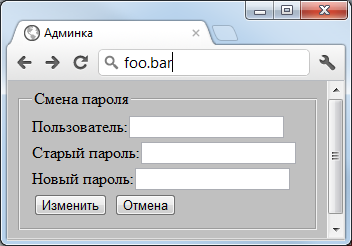
\includegraphics[width=0.6\textwidth]{fig/htmform.png}
    }
    \only<2>{
        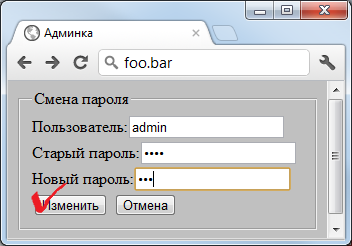
\includegraphics[width=0.6\textwidth]{fig/htmformclick.png}
    }
    
    \uncover<2>{
Броузер сформирует запрос серверу \verb"foo.bar":
\begin{semiverbatim}    
GET /pwdscrypt.jsp?\alert{login=admin}\&\alert{oldpw=fool}\&\alert{newpw=god}
\end{semiverbatim}    
    }
\end{frame}

\begin{frame}[fragile]
    \frametitle{SQL-injection}
    \framesubtitle{Обработка запроса сервером \verb"foo.bar". JSP-технология. pwdscrypt.jsp}
        
    \shorthandoff{"}
    \begin{semiverbatim}
<%page import="java.sql.*"%>
<HTML> 
  <HEAD> <TITLE>Результат обновления пароля</TITLE>
    <META CONTENT="text/html;charset=windows-1251"></HEAD>
  <BODY BGCOLOR="silver">
<%
\alert<2>{try \{ //Уязвимый фрагмент серверного кода. Обращение к БД
}%>
    <p>success!!!</p>
<%
\alert<2>{\} catch(Exception e) \{System.err.println(e.getMessage());\}}
%>
  </BODY>
</HTML>
    \end{semiverbatim}
    \shorthandon{"}
\end{frame}


\begin{frame}[fragile]
    \frametitle{SQL-injection}
    \framesubtitle{Уязвимый фрагмент серверного кода. Обращение к БД}
    
    \shorthandoff{"}
    \begin{semiverbatim}
String driver = "org.gjt.mm.mysql.Driver";
String url    = "jdbc:mysql://localhost/sqlinjtest";
Class.forName(driver);
Connection conn = DriverManager.getConnection(url);

Statement stmt = conn.createStatement();
\alert<2>{String    sql  = 
    "update profile set"
    + " password=\\"" + request.getParameter("newpw") + "\\""
    + " where"
    + " login=\\""    + request.getParameter("login") + "\\""
    + " and pass=\\"" + request.getParameter("oldpw") + "\\"";}
stmt.executeUpdate(\alert<2>{sql});
conn.close();
    \end{semiverbatim}
    \shorthandon{"}
\end{frame}

\begin{frame}[fragile]
    \frametitle{SQL-injection}
    \framesubtitle{Нормальное развитие ситуации}
    
    В приведенном примере будет сгенерирована следующая строка запроса (переносы добавлены для удобочитаемости):
    \shorthandoff{"}
    \begin{semiverbatim}
update profile set pass="god" 
  where login="admin" and pass="fool"
    \end{semiverbatim}
    \shorthandon{"}
    Счастливый пользователь узнает, что все прошло как надо:
    
    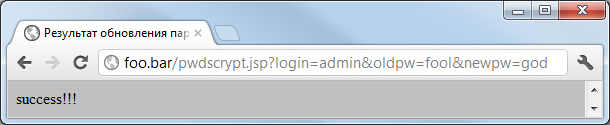
\includegraphics[width=\textwidth]{fig/htmrespok.png}
\end{frame}

\begin{frame}[fragile]
    \frametitle{SQL-injection}
    \framesubtitle{Внедрение}
    
    Если вместо имени пользователя злоумышленник вводит сторку
    \shorthandoff{"}
\begin{verbatim}
admin" or 2>1 --
\end{verbatim}
    \shorthandon{"}
    
    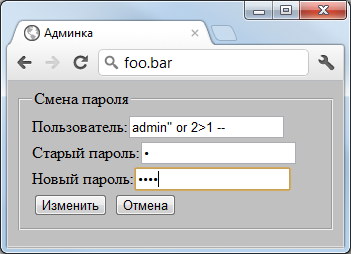
\includegraphics[width=0.4\textwidth]{fig/htmlformhack.png}
    
    и браузер шлёт запрос:
\begin{verbatim}
/pwdscrypt.jsp?
  login=admin%22+or+2%3E1+--&oldpw=%3F&newpw=fail
\end{verbatim}
\end{frame}


\begin{frame}[fragile]
    \frametitle{SQL-injection}
    \framesubtitle{Внедрение}
    
    то уязвимым скриптом будет сгенерирована следующая строка запроса к БД (переносы добавлены для удобочитаемости):
    \shorthandoff{"}
    \begin{semiverbatim}
update profile set pass="fail" 
  where login="admin" or 2>1 \only<1-2>{\alert<2>{{-}- and pass="?"}}
    \end{semiverbatim}
    \shorthandon{"}
    
    \uncover<3>{Нетрудно предсказать результаты выполнения данного запроса.}
\end{frame}


\begin{frame}
    \frametitle{SQL-injection}
    \framesubtitle{Признаки уязвимости}
    
    Уязвим любой язык программирования, позволяющий обращения с запросами к БД.
    
    Признаки узязвимости в серверном коде.
    \begin{enumerate}
        \item Код использует ввод пользователя.
        \item Код не проверяет ввод пользователя.
        \item Код использует пользовательские данные для построения запроса к базе данных.
        \item Код использует конкатенацию строк для построения запроса.
    \end{enumerate}
\end{frame}

\begin{frame}
    \frametitle{SQL-injection}
    \framesubtitle{Как бороться?}
    
    \begin{enumerate}
        \item Не использовать конкатенацию строк для формирования запроса!
        \item Использовать prepared statements --- параметризованные подготовленные запросы.
        \item В крайнем случае использовать квотирование значений параметров запроса (т.е. использовать принятое в БД кодирование SQL-спецсимволов как части строкового значения).
        \item Шифровать конфиденциальные данные в БД.
    \end{enumerate}
\end{frame}

    
\subsection{XSS/XSRF}

\begin{frame}
    \frametitle{Типы XSS}
    
    \alert{XSS --- Сross Site Sсriрting}. Целью XSS-атак является броузер клиента и хранимая им информация\footnote{Чаще всего cookies или скрытые элементы в DOM страницы}. Выделяют следующие типы XSS.
    \begin{itemize}
        \item Тип 0. Атаки XSS на базе DOM.
        \item Тип 1. Отраженные XSS. 
        \item Тип 2. Сохраненные XSS.
    \end{itemize}
    
    Атаки XSS основаны на чрезмерном доверии клиента к серверу.
\end{frame}

\begin{frame}
    \frametitle{Типы XSS}
    \framesubtitle{Атаки XSS на базе DOM}

    \alert{Атаки XSS на базе DOM}.
    
    Пользователь должен зайти на страницу злоумышленника, которая содержит html-код (в т.ч. скрипты), использующий бреши в реализации DOM\footnote{DOM --- Document Object Model} браузером.
\end{frame}

\begin{frame}[fragile]
    \frametitle{Типы XSS}
    \framesubtitle{Отраженные XSS}

    \shorthandoff{"}
    \alert{Отраженные XSS}. 
    \begin{itemize}
        \item Разработчик пишет небезопасный серверный код, который дублирует на странице параметры запроса клиента.
        \item Злоумышленник, выявив уязвимость, встраивает в запрос серверу вредоносный клиентский код\footnote{Чаще всего JavaScript}. И добивается того, чтобы пользователь выполнил этот запрос\footnote{Например, посылает ссылку со сформированным GET-запросом по почте (теги {<}a href="url"{>}, {<}img src="url"{>}), оставляет ссылку в комметнариях на форуме и т.д.}.
        \item Пользователь, выполнив запрос, получает от сервера страницу, содержащую вредоносный скрипт злоумышленника, который и выполняется броузером пользователя.
    \end{itemize}
\end{frame}


\begin{frame}
    \frametitle{Типы XSS}
    \framesubtitle{Сохраненные XSS}

    \alert{Сохраненные XSS}. 
    \begin{itemize}
        \item Разработчик пишет небезопасный серверный код, который сохраняет непроверенные данные\footnote{Что необходимо для организации форумов, блогов, чатов и пр\ldots} запроса клиента, а также использует сохраненные данные для формирования контента страницы, не выполняя никаких проверок.
        
        \item Злоумышленник, выявив уязвимость, встраивает в запрос серверу вредоносный клиентский код и выполняет его.
        
        \item Пользователь, зайдя на сайт, подвергшийся атаке, получает страницу, содержащую вредоносный скрипт злоумышленника, который и выполняется броузером.
    \end{itemize}
\end{frame}

\begin{frame}
    \frametitle{Пример XSS-узявимости}
    
    Рассмотрим надуманный пример отраженного XSS. Пользователь вводит свое имя в форме, а сервер отвечает приветствием. 
    
\end{frame}

\begin{frame}[fragile]
    \frametitle{Пример XSS-узявимости}
    \framesubtitle{Страница приветствия}
    
    \shorthandoff{"}
    \begin{semiverbatim}
<HTML> 
  <HEAD> <TITLE>Представьтесь</TITLE>
     <META CONTENT="text/html; charset=windows-1251"></HEAD>
  <BODY BGCOLOR="silver">
     <FORM action="hello.jsp">
        <FIELDSET>  <LEGEND>Немного о себе</LEGEND>
           Моё имя:<INPUT TYPE="text" NAME="name"><BR>
           Мой ник:<INPUT TYPE="text" NAME="nickname"><BR>
           <INPUT TYPE="submit" VALUE="Представиться"> 
           <INPUT TYPE="reset" VALUE="Отмена"><BR>
        </FIELDSET>
     </FORM>
  </BODY>
</HTML>
    \end{semiverbatim}
    \shorthandon{"}
\end{frame}

\begin{frame}[fragile]
    \frametitle{Пример XSS-узявимости}
    \framesubtitle{Запрос серверу}
    
    \only<1>{
        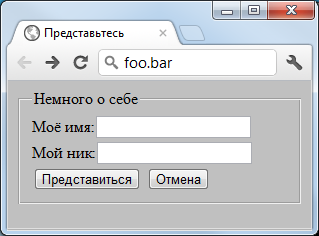
\includegraphics[width=0.6\textwidth]{fig/htmlxss.png}
    }
    \only<2>{
        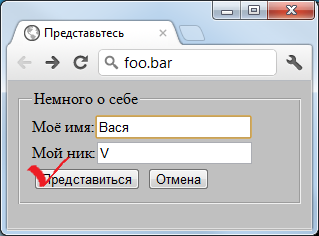
\includegraphics[width=0.6\textwidth]{fig/htmlxssclick.png}
    }
    
    \uncover<2>{
Броузер сформирует запрос серверу \verb"foo.bar":
\begin{semiverbatim}    
GET /hello.jsp?\alert{name=\%C2\%E0\%F1\%FF}\&\alert{nickname=V}
\end{semiverbatim}    
    }
\end{frame}

\begin{frame}[fragile]
    \frametitle{Пример XSS-узявимости}
    \framesubtitle{Обработка запроса сервером \verb"foo.bar". JSP-технология. hello.jsp}
        
    \shorthandoff{"}
    \begin{semiverbatim}
<HTML> 
  <HEAD> <TITLE>Приветствие</TITLE>
    <META CONTENT="text/html;charset=windows-1251"></HEAD>
  <BODY BGCOLOR="silver">
    К нам приехал, к нам приехал, 
    <%= \alert{request.getParameter("name")} %> 
    ака <%= \alert{request.getParameter("nickname")} %>,
    да-а-а-рагой!!!
  </BODY>
</HTML>
    \end{semiverbatim}
    \shorthandon{"}
\end{frame}

\begin{frame}[fragile]
    \frametitle{Пример XSS-узявимости}
    \framesubtitle{Нормальное развитие ситуации}
    
    Счастливый пользователь получает приветствие:
    
    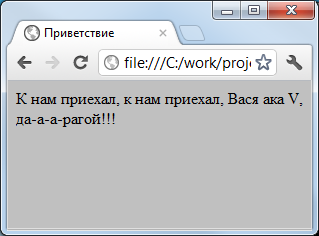
\includegraphics[width=0.6\textwidth]{fig/htmlxssok.png}
\end{frame}

\begin{frame}[fragile]
    \frametitle{Пример XSS-узявимости}
    \framesubtitle{Выявление угрозы}
    
    Если вместо имени пользователя злоумышленник вводит сторку, например
    \shorthandoff{"}
\begin{semiverbatim}
Вася\alert{ <script>alert("Evil code!")</script>}
\end{semiverbatim}
    , то браузер пошлёт запрос:
\begin{verbatim}
/hello.jsp?
    name=%C2%E0%F1%FF
        %3Cscript%3E
            alert%28%22Evil+code%21%22%29
        %3C%2Fscript%3E
    \&nickname=V
\end{verbatim}
    \shorthandon{"}
\end{frame}

\begin{frame}[fragile]
    \frametitle{Пример XSS-узявимости}
    \framesubtitle{Выявление угрозы}
    
    В ответ на запрос браузер получит от сервера следующий html-код
    \shorthandoff{"}
\begin{semiverbatim}
<HTML>
  <HEAD> <TITLE>Приветствие</TITLE>
    <META CONTENT="text/html;charset=windows-1251"></HEAD>
  <BODY BGCOLOR="silver">
    К нам приехал, к нам приехал, 
    Вася<script>alert("Evil code!")</script>
    ака V,
    да-а-а-рагой!!!
  </BODY>
</HTML>
\end{semiverbatim}
    \shorthandon{"}
\end{frame}

\begin{frame}[fragile]
    \frametitle{Пример XSS-узявимости}
    \framesubtitle{Выявление угрозы}

    и выполнит скрипт:
    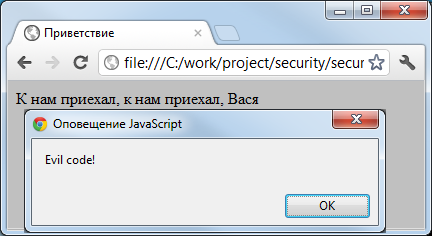
\includegraphics[width=0.8\textwidth]{fig/htmlxsshack.png}
\end{frame}

\begin{frame}[fragile]
    \frametitle{Пример XSS-узявимости}
    \framesubtitle{Атака}

    Злоумышленнику достаточно, например, опубликовать на доверенном сайте ссылку (переносы в значении href добавлены для удобочитаемости):
    \shorthandoff{"}
\begin{verbatim}
  <a href="http://foo.bar/hello.jsp?
      name=%C2%E0%F1%FF
        %3Cscript%3E
          alert%28%22Evil+code%21%22%29
        %3C%2Fscript%3E
      &nickname=V">
    Это стоит видеть
  </a>
\end{verbatim}
    \shorthandon{"}
    Реальный Evil code будет, например, похищать параметры сессии пользователя.
\end{frame}


\begin{frame}
    \frametitle{XSS}
    \framesubtitle{Признаки уязвимости}
    
    Уязвим практически любой язык web-программирования.
    
    Признаки узязвимости в серверном коде.
    \begin{enumerate}
        \item Код использует параметры http-запроса.
        \item Код не проверяет используемые параметры.
        \item Код использует параметры для формирования web-страницы.
    \end{enumerate}
\end{frame}

\begin{frame}
    \frametitle{XSS}
    \framesubtitle{Как бороться?}
    
    \begin{enumerate}
        \item Проверять корректность параметров запроса.
        \item Примененять защитное кодирование (xml/html encode).
        \item Удалять из входных данных комбинации CRLF, если эти данные используются для формирования http-заголовка.
    \end{enumerate}
\end{frame}


\begin{frame}
    \frametitle{Кратко о XSRF}
    \framesubtitle{Суть проблемы}

    XSRF (Сross Site Request Forgery\footnote{Межсайтовая фальсификация запросов}) основаны на избытке доверия сервера к клиенту.

    XSRF (также называемые CSRF) представляют собой ошибки проектирования приложения, и с недостаточным контролем ввода никак не связаны. XSRF проявляются, если пользователь может отсылать в запросах инструкции управления серверным приложением.
    \begin{enumerate}
        \item Пользователь проходит аутентификацию.
        \item Пользователь открывает страницу (сформированную злоумышленником\footnote{Хорошие примеры: блог-площадки, форумы, почтовые web-интерфейсы и т.д.}), содержащую ссылку или формирующую запрос с инструкцией управления.
        \item Сервер, доверяя аутентичному пользователю, выполняет инструкцию.
    \end{enumerate}
\end{frame}

\begin{frame}
    \frametitle{XSRF}
    \framesubtitle{Как бороться?}

    \begin{enumerate}
        \item Добавить секретное значение <<ключ>> для сеанса между клиентом и сервером; это значение не должно включаться в cookie.
        \item Реализовать тайм-аут в сеансе. Тайм-аут защищается MAC\footnote{Message Authentication Code}.
        \item Желательно использовать POST-запросы.
    \end{enumerate}
    
    Важно знать, что единственный деффект XSS позволит обойти защитные меры от XSRF.
\end{frame}



\section{Защита}

\subsection{Защита от срыва стека}


\begin{frame}
    \frametitle{Защита от срыва стека}
    
    Далее рассматриваются элементы встраиваемых защит от срыва стека.
    \begin{enumerate}
        \item Проверка факта переполнения и завершение программы.
        \item Разделение стеков. Программно эмулируется стек для сохранения адресов возврата.
        \item Копирование аргументов-указателей\footnote{Например, указатели на функции или объекты, для которых выполняется вызов член-функций} в локальные переменные на вершине стека.
        \item и т.д.
    \end{enumerate}
\end{frame}


\begin{frame}[fragile]
    \frametitle{Защита от срыва стека}
    \framesubtitle{Проверка переполнения. Исходный вариант}

\shorthandoff{"}
\begin{columns}
    \column{0.6\textwidth}
\begin{semiverbatim}
void foo(arg1, arg2) \{
    int   scalar1;
    int  *scalar2;
    char buf1[BUF_SIZE1];
    char buf2[BUF_SIZE2];

    bar1(...);
    \alert{gets(buf2)};
    bar2(...);
\}
\end{semiverbatim}
    \column{0.3\textwidth}
        \begin{block}{}
\begin{semiverbatim}
[buf2        ...]
[buf1        ...]
[scalar2     ]
[scalar1     ]
[ebp         ]
[ret address ]
[arg1        ]
[arg2        ]
\end{semiverbatim}
        \end{block}
\end{columns}
\shorthandon{"}
\end{frame}


\begin{frame}[fragile]
    \frametitle{Защита от срыва стека}
    \framesubtitle{Проверка переполнения. Защита (\alert{выделен} код, добавленный защитой)}

\shorthandoff{"}
\begin{columns}
    \column{0.6\textwidth}
\begin{semiverbatim}
\alert{unsigned int guard_value=magic};
void foo(arg1, arg2) \{
\alert{    volatile unsigned int guard};
    char buf1[BUF_SIZE1];
    char buf2[BUF_SIZE2];
    int   scalar1;
    int  *scalar2;

\alert{    \only<2>{->}guard=guard_value};
    bar1(...);
    \only<3>{->}gets(buf2);
    bar2(...);
\alert{    \only<4>{->}if (guard != guard_value) halt()};
\}
\end{semiverbatim}
    \column{0.3\textwidth}
        \begin{block}{}
\begin{semiverbatim}
[scalar2     ]
[scalar1     ]
\only<1,2>{[buf2        ...]}\only<3->{[\alert{evil} buf2   ...]}
\only<1,2>{[buf1        ...]}\only<3->{[\alert{evil} buf1   ...]}
\only<1>{[guard=???   ]}\only<2>{[guard=\alert{magic} ]}\only<3,4>{[guard=\alert{evil}  ]}
\only<1,2>{[ebp         ]}\only<3->{[\alert{evil} ebp    ]}
\only<1,2>{[retaddr     ]}\only<3->{[\alert{evil} retaddr]}
\only<1,2>{[arg1        ]}\only<3->{[\alert{evil} arg1   ]}
\only<1,2>{[arg2        ]}\only<3->{[\alert{evil} arg2   ]}
\end{semiverbatim}
        \end{block}
\end{columns}
\shorthandon{"}
\end{frame}


\begin{frame}[fragile]
    \frametitle{Защита от срыва стека}
    \framesubtitle{Альтернативный стек. Исходный вариант}

\shorthandoff{"}
\begin{columns}
    \column{0.6\textwidth}
\begin{semiverbatim}
void foo(arg1, arg2) \{
    char buf[BUF_SIZE];
    
    bar1(...);
    \alert{gets(buf)};
    bar2(...);
\}
\end{semiverbatim}
    \column{0.3\textwidth}
        \begin{block}{}
\begin{semiverbatim}
[buf        ...]
[ebp         ]
[ret address ]
[arg1        ]
[arg2        ]
\end{semiverbatim}
        \end{block}
\end{columns}
\shorthandon{"}
\end{frame}


\begin{frame}[fragile]
    \frametitle{Защита от срыва стека}
    \framesubtitle{Альтернативный стек. Защита (\alert{выделен} код, добавленный защитой)}

\shorthandoff{"}
\begin{columns}
    \column{0.6\textwidth}
\begin{semiverbatim}
\alert{unsigned int altSp};
\alert{void *altStack[ALT_STACK_SIZE]};

void foo(arg1, arg2) \{
    char buf[BUF_SIZE];
    
\alert{    \only<2>{->}altPush()};
    bar1(...);
    \only<3>{->}gets(buf);
    bar2(...);
\alert{    \only<4>{->}altPop()};
\}
\end{semiverbatim}
    \column{0.3\textwidth}
        \begin{block}{altStack}
\begin{semiverbatim}
\only<2-3>{[good retaddr]}
[............]
\end{semiverbatim}
        \end{block}
        \begin{block}{}
\begin{semiverbatim}
[buf        ...]
\only<1,2>{[ebp         ]}\only<3,4>{[\alert{evil} ebp    ]}
\only<1,2,4>{[good retaddr]}\only<3>{[\alert{evil} retaddr]}
\only<1,2>{[arg1        ]}\only<3,4>{[\alert{evil} arg1   ]}
\only<1,2>{[arg2        ]}\only<3,4>{[\alert{evil} arg2   ]}
\end{semiverbatim}
        \end{block}
\end{columns}
\shorthandon{"}
\end{frame}


\subsection{PCRE}

\begin{frame}
    \frametitle{PCRE}
    \framesubtitle{Perl Compatible Regular Expressions}
    
    В составе PCRE выделяют:
    \begin{itemize}
        \item одиночные символы; 
        \item классы символов; 
        \item альтернативы; 
        \item квантификаторы; 
        \item мнимые символы; 
        \item ссылки на найденный текст;
        \item и т.д.
    \end{itemize}
\end{frame}

\begin{frame}
    \frametitle{PCRE}
    \framesubtitle{Одиночный символ}
    
    Любой одиночный символ $s$ в составе PCRE соответствует сам себе, если только он не является служебным символом (спецсимволом), играющим особую роль. 
    
    Служебными символами являются <<\textbackslash>>, <<|>>, <<(>>, <<)>>, <<[>>, <<]>>, <<\{>>, <<\}>>, <<*>>, <<+>>, <<\^{}>>, <<\$>>, <<?>> и <<.>>. 
    
    Если необходимо, чтобы служебный символ соответствовал самому себе, то перед ним нужно поставить символ <<\textbackslash>>. Регулярное выражение, производящее поиск символа <<\textbackslash>> в тексте будет выглядеть так <<\textbackslash\textbackslash>>.
\end{frame}

\begin{frame}
    \frametitle{PCRE}
    \framesubtitle{Предопределенные классы и символы, ввод которых затруднён}
    
    \begin{itemize}
        \item{} <<\textbackslash d>> – любая десятичная цифра;
        \item{} <<\textbackslash D>> – любой символ, кроме десятичной цифры;
        \item{} <<\textbackslash s>> – любой из символов-разделителей;
        \item{} <<\textbackslash S>> – любой символ, за исключением пробельного;
        \item{} <<\textbackslash w>> – алфавитно-цифровой символ и знак <<\_>>;
        \item{} <<\textbackslash W>> – любой символ, но не <<\textbackslash w>>;
        \item{} <<\textbackslash r>>  – символ перевода каретки <CR>;
        \item{} <<\textbackslash n>>  – символ новой строки <LF>;
        \item{} <<\textbackslash R>>  – независимый от платформы разделитель строк;
        \item{} <<\textbackslash xHH>> – символ ASCII с кодом из двух шестнадцатеричных (HH) цифр;
        \item{} <<\textbackslash uHHHH>> – символ Unicode с кодом из четырех шестнадцатеричных (HHHH) цифр.
    \end{itemize}
\end{frame}

\begin{frame}
    \frametitle{PCRE}
    \framesubtitle{Точка}

    Спецсимвол точка <<.>> соответствует любому символу, за исключением разделителя строк.
\end{frame}

\begin{frame}
    \frametitle{PCRE}
    \framesubtitle{Классы символов}
    
    \alert{Класс} определяет соответствие одному символу из множества. Класс --- это список символов, заключенный в квадратные скобки <<[>>, <<]>>. Можно указать как отельные символы, так и диапазон. Диапазон задается двумя крайними символами диапазона, разделенными тире. Если требуется указать тире, то перед ним ставится символ <<\textbackslash>>. 
    
    Например.
    \begin{itemize}
        \item{} <<[abcde]>> --- любая из букв <<а>>, <<b>>, <<c>>, <<d>>, <<e>>. Более кратко: <<[a-e]>>.
        \item Равнозначны: <<[\textbackslash-0123456789]>>, <<[\textbackslash-0-9]>> и <<[\textbackslash-\textbackslash d]>>.
    \end{itemize}
     Если сразу после открывающей квадратной скобки следует спецсимвол <<\^{}>>, то будет выполняться поиск соответствия символу, не входящему в класс. Например, <<[\^{}a-e]>> --- любой символ, \emph{кроме}: <<а>>, <<b>>, <<c>>, <<d>>, <<e>>.
\end{frame}


\begin{frame}
    \frametitle{PCRE}
    \framesubtitle{Альтернативы}
    
    \alert{Альтернативa} соответствуют операции объединения в формальном определении регулярных выражений. Альтернативные регулярные выражения разделяются спецсимволом <<|>> и обычно заключаются в круглые скобки.

    Альтернатива <<(a|b)>> соответствует либо шаблону <<a>>, либо <<b>>.
    
    Например.
    \begin{enumerate}
        \item Двоичная цифра: <<(0|1)>>.
        \item Троичная цифра: <<(0|1|2)>>.
        \item Любая тетрада:  <<(0|1)(0|1)(0|1)(0|1)>>.
        \item Четыре варианта резьбы по дереву\footnote{Экономный троллинг}: <<(саша|паша)\textbackslash+(маша|даша)=Л>>.
    \end{enumerate}
\end{frame}


\begin{frame}
    \frametitle{PCRE}
    \framesubtitle{Квантификаторы}
    
    \alert{Квантификаторы} ставятся после регулярного выражения и определяют количество повторений шаблона. Выделяют следующие квантификаторы:
    \begin{itemize}
        \item{} <<*>> --- ноль или несколько повторов;
        \item{} <<+>> --- один или несколько повторов;
        \item{} <<?>> --- ноль или один повтор;
        \item{} <<\{$n$\}>> --- ровно $n$ повторов;
        \item{} <<\{$n$,\}>> --- по крайней мере $n$ повторов;
        \item{} <<\{$n$,$m$\}>> --- от $n$ до $m$ повторов.
    \end{itemize}
\end{frame}

\begin{frame}
    \frametitle{PCRE}
    \framesubtitle{Жадность и лень}
    
    По умолчанию квантификаторы <<*>>, <<+>>, <<?>>, <\{$n$,\}>>, <<\{$n$,$m$\}>> являются \alert{жадными} (greedy): они выделят по возможности самый длинный фрагмент из всех возможных. 
    
    Например, при поиске в тексте <<aaaaaaaaaa>> шаблону <<a*a>> будет соответствовать весь текст. Сделать квантификаторы \alert{ленивыми} (lazy) можно, поставив после них знак вопроса <<?>>. Тогда в приведенном примере для <<ленивого>> варианта <<a*?a>> результатом поиска будет одна буква <<a>>.    
\end{frame}


\begin{frame}
    \frametitle{PCRE}
    \framesubtitle{Мнимые символы}
    
    \alert{Мнимые символы} не соответствуют символам текста! Они соответствуют выполнению определенного условия (assertion), например:
    \begin{itemize}
        \item{} <<\^{}>> --- начало строки текста;
        \item{} <<\$>> --- конец строки или позиция перед символом начала новой строки;
        \item{} <<\textbackslash b>> --- граница слова;
        \item{} <<\textbackslash B>> --- отсутствие границы слова.
    \end{itemize}
\end{frame}


\begin{frame}
    \frametitle{PCRE}
    \framesubtitle{Сылки на фрагменты шаблона}
    
    Каждому выражению, заключенному в скобки соответствует переменная с определенным номером. Так как части регулярного выражения заключенные в скобки могут быть вложенными, то нумеруются они с единицы по открывающим скобкам, слева направо. В 0-й переменной содержится текст соответствующий шаблону целиком.
    
    Например, если задано регулярное выражение <<(\textbackslash w(\textbackslash w(\textbackslash w)))((\textbackslash w)(\textbackslash w))>> и текст <<ABCDE>>, то значения переменных будут: \$0=<<ABCDE>>, \$1=<<ABC>>, \$2=<<BC>>, \$3=<<C>>, \$4=<<DE>>, \$5=<<D>>, \$6=<<E>>. 
\end{frame}

\begin{frame}[fragile]
    \frametitle{PCRE}
    \framesubtitle{Поиск со ссылками на найденные фрагменты}
    
    Иногда в процессе поиска нужно сослаться на подстроку текста, для которой уже получено совпадение с некоторой частью регулярного выражения. 
    
    Для этого необходимую часть следует заключить в круглые скобки и сослаться на нее. Для этого перед номером переменной достаточно поставить <<\textbackslash>>. 
    
    Например, если вы желаете найти целое положительное число, являющееся значением элемента XML\footnote{Например: \verb"some text <age>100</age> some text"}, то вы можете задать такое выражение: << <(\textbackslash w+)>\textbackslash d+</\textbackslash 1> >>. В переменной \textbackslash 1 будет содержаться текст, который был найден как соответствующий регулярному выражению <<(\textbackslash w+)>>.    
\end{frame}

\begin{frame}
    \frametitle{PCRE}
    \framesubtitle{Замены}
    
    С помощью ссылок на фрагменты текста, соответствующего шаблону регулярного выражения очень удобно выполнять самые нетривиальные замены в тексте. Например, переставить байты в 32 битном шестнадцатеричном числе в обратном порядке можно так: заменить текст, соответствующий регулярному выражению 
    \[
    \text{<<0x([0-9a-fA-F]\{2\})([0-9a-fA-F]\{2\})([0-9a-fA-F]\{2\})([0-9a-fA-F]\{2\})>>}
    \]
    на текст\footnote{Здесь мы обращаемся к переменной с номером n так <<\$n>>} <<0x\$4\$3\$2\$1>>. Число <<0x01ABCDEF>> будет заменено на <<0xEFCDAB01>>.
\end{frame}
    
\begin{frame}
    \frametitle{PCRE}
    \framesubtitle{Есть в любом стоящем текстовом редакторе. В IDE и подавно}
    \begin{figure}
        \centering
        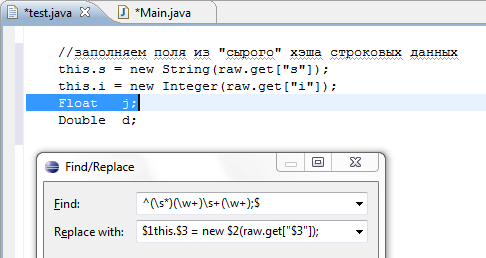
\includegraphics[width=\textwidth]{fig/eclipseIde}
    \end{figure} 
\end{frame}
    
\appendix


%сводка по ссылкам
\begin{frame}
    \frametitle{Источники}
    
    Рекомендуется к прочтению книга \cite{bib:howard:24}. Доступно о защите от срыва стека см. \cite{bib:misch:stackProt}.
\end{frame}


%слайд раскладывается на несколько: allowframebreaks
\begin{frame}[allowframebreaks]{Библиография}
    \bibliographystyle{gost780u}
    \bibliography{./../bibliobase}
\end{frame}


\end{document}